\documentclass[aspectratio=1610, 13pt]{beamer}
\usepackage{xcolor}
\usepackage{multicol}
\usepackage{mathtools,array}
\usepackage[T1]{fontenc}

\usepackage{stmaryrd}
\usepackage{dutchcal}
\usepackage{zi4}
\usepackage[font={scriptsize,bf}]{caption}
% \usepackage{subcaption}
\usepackage{graphics}
\usepackage{tikz}
\usepackage{fontawesome5}
\usepackage{mathpartir}

\newcommand{\naturals}{\mathbb{N}}
\newcommand{\reals}{\mathbb{R}}

\newcommand{\Dist}[1]{\mathcal{D}(#1)}
\newcommand{\expectation}{\mathbb{E}}

\newcommand{\states}{S}
\newcommand{\actions}{A}
\newcommand{\observables}{O}
\newcommand{\trans}{T}
\newcommand{\obs}{Z}
\newcommand{\reward}{R}
\newcommand{\discount}{\gamma}

\newcommand{\beliefs}{\mathcal{B}}
\newcommand{\beliefUpdate}{\tau}

\newcommand{\policy}{\pi}

\newcommand{\diff}[1]{\mathop{}\!\mathrm{d}#1}
\renewcommand{\figurename}{Figure}
\renewcommand{\refname}{Reference}

\AtBeginDocument{
  \catcode`_=12
  \begingroup\lccode`~=`_
  \lowercase{\endgroup\let~}\sb
  \mathcode`_="8000
}

% \usetheme{Madrid}
% % \usetheme{default}
% \setbeamertemplate{caption}[numbered]
% \setbeamerfont{title}{size=\large}
\mode<presentation>
{
  \usetheme{Darmstadt}      % or try Darmstadt, Madrid, Warsaw, ...
  \usecolortheme{default} % or try albatross, beaver, crane, ...
  \usefonttheme[onlymath]{serif}  % or try serif, structurebold, ...
  \setbeamertemplate{navigation symbols}{}
  \setbeamertemplate{caption}[numbered]
  \setbeamertemplate{footline}[frame number] 
} 

\usepackage{listings}
\lstdefinestyle{heaplang}{
    language=Caml,
    basicstyle=\footnotesize\ttfamily,
    keywordstyle=\color{blue},
    commentstyle=\color{red},
    escapeinside={<@}{@>},
    morekeywords={new_chan, fork, recv, send, swap, ref}
}
\lstdefinestyle{clang}{
    language=Caml,
    basicstyle=\footnotesize\ttfamily,
    keywordstyle=\color{blue},
    commentstyle=\color{red},
    escapeinside={<@}{@>},
}
\lstset{style=heaplang}

\usepackage{natbib}

\newcommand{\buchi}{B\"uchi }

\definecolor{goldenpoppy}{rgb}{0.99, 0.76, 0.0}
\definecolor{goldenyellow}{rgb}{1.0, 0.87, 0.0}
\definecolor{green2}{rgb}{0.1,0.7,0.3} 
\newcommand{\gcheck}{{\color{green2}\faCheckCircle[regular] }}
\newcommand{\rcross}{{\color{red} \faTimesCircle[regular]} }
\newcommand{\rflag}{{\color{red} \faFlag}}
% \usepackage{algorithm,amsmath}
% \usepackage[noend]{algpseudocode}

\newcommand{\zlstinline}{\let\par\endgraf\lstinline}
\newcommand{\comments}[1]{{\color{red}#1}}
\title{Chapter 6: Algorithms}
\author{Reporter:  Xie Li}
\date{\today}
\begin{document}
\maketitle

\begin{frame}{Overview}
\begin{itemize}
\item [6.1] Abstract  worklist algorithm.
\item [A.C] Preliminaries.
\item [6.2] Iterating in reverse postorder.
\item [6.3] Iterating through strong components.
\end{itemize}
\end{frame}

\begin{frame}
\begin{center}
\Large
\textbf{Part I: Abstract Worklist Algorithm}
\end{center}
\end{frame}

\begin{frame}{Worklist Algorithm: Reaching Definition Analysis Example}

\begin{center}
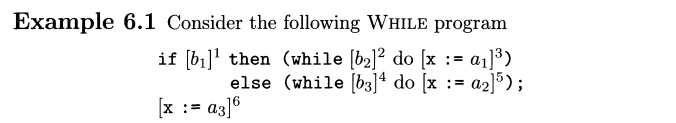
\includegraphics[scale=0.4]{rdexp.png}

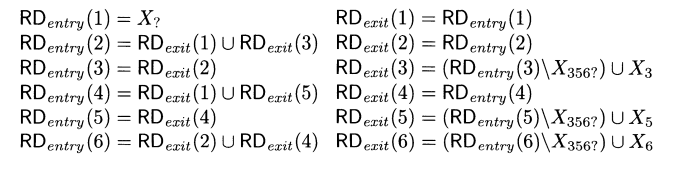
\includegraphics[scale=0.4]{rdexp1.png}
\end{center}

\begin{center}
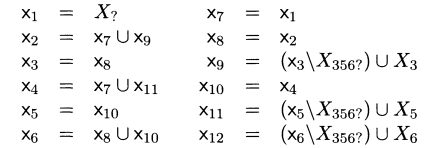
\includegraphics[scale=0.4]{rdexp2.png}
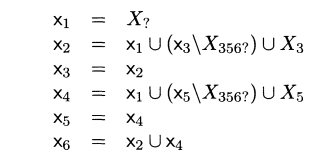
\includegraphics[scale=0.4]{rdexp3.png}
\end{center}

where $\mathbf{X}_{356?}$ represents $\{(x, 3), (x, 5), (x, 6), (x, ?)\}$

\end{frame}


\begin{frame}{Assumptions}
\textbf{Assumptions:}
\begin{itemize}
\item A finite contraint system $(x_i \sqsupseteq t_i)_{i = 1}^N$, where $N \ge 1$
\item  $\bigcup_i\text{FV}(t_i) \subseteq X = \{x_i\ \mid  1 \le i \le N\}$
\item A solution is a total function $\psi: X \rightarrow L$, where $(L, \sqsubseteq)$ is a complete lattice satisfying the Acending Chain Condition.
\item Terms are interpreted by the solutions. $\llbracket t\rrbracket \psi\in L$.
\item The interpretation $\llbracket t\rrbracket \psi$ of a term $t$ is monotone in $\psi$ and its value only depends on the values $\{\psi(x) \mid x \in \text{FV}(t)\}$
\end{itemize}


\textbf{Equations vs. inequations}:
\[x \sqsupseteq t_1, \ldots x \sqsupseteq t_n\]
and 
\[x = x \sqcup t_1 \sqcup \ldots \sqcup t_n\]
have the same solutions, and the least solution of the system is also the least solution of 
\[x =  t_1 \sqcup \ldots \sqcup t_n\]
\end{frame}


\begin{frame}{Abstract Worklist Algorithms}
\begin{multicols}{2}
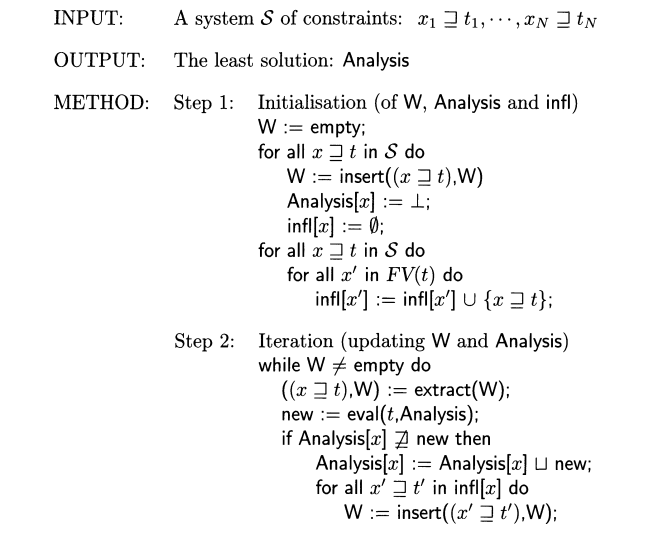
\includegraphics[scale=0.4]{absAlgo.png}

\end{multicols}
\end{frame}

\begin{frame}{Abstract Worklist Algorithm}
\begin{center}

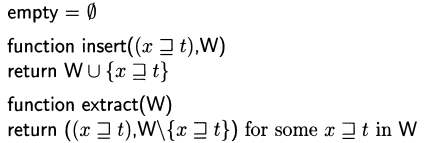
\includegraphics[scale=0.4]{absAlgo1.png}
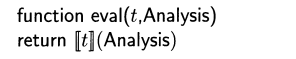
\includegraphics[scale=0.4]{absAlgo2.png}
\end{center}
and 
\[\texttt{infl}[x] = \{(x' \sqsupseteq t')\in \mathcal{S} \mid x \in \text{FV}(t')\}\]
\textbf{Example of influence:}
\begin{center}

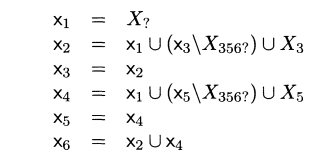
\includegraphics[scale=0.4]{rdexp3.png}
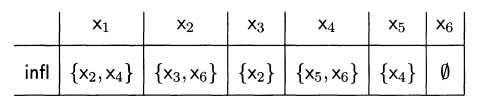
\includegraphics[scale=0.4]{infl.png}
\end{center}
\end{frame}

\begin{frame}{Properties of the Algorithm}
Given a contraint system $\mathcal{S} = (x_i \sqsupseteq t_i)_{i = 1}^N$, we define a function
\[F_{\mathcal{S}}:(X\rightarrow L) \rightarrow (X\rightarrow L)\]
by
\[F_{\mathcal{S}}(\phi)(x) = \bigsqcup \{\llbracket t \rrbracket \phi \mid x \sqsupseteq t \text{ in }\mathcal{S}\}\]

This defines a monotone function over complete lattice $X \rightarrow L$
\begin{itemize}
\item Monotone: can be checked easily. $\phi \sqsubseteq \psi \Rightarrow {F}_{\mathcal{S}}(\phi) \sqsubseteq {F}_{\mathcal{S}}(\psi)$
\item Ascending chain condition: $X$ is finite and $L$ by assumption satisfies ascending chain condition...
\end{itemize}
\end{frame}

\begin{frame}{Correctness of the Algorithm}
\begin{lemma}[6.4]

Given the assumptions, the abstract algorithm computes the least solution of the given contraint system, $\mathcal{S}$.



\end{lemma}
\begin{proof}
\begin{multicols}{2}
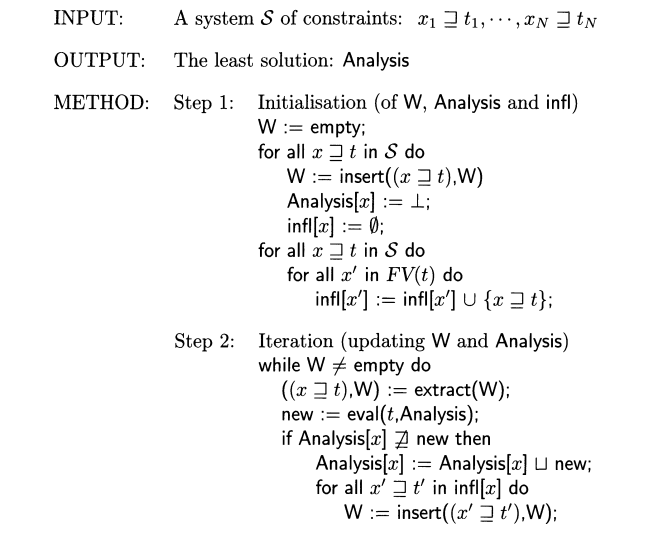
\includegraphics[scale=0.27]{absAlgo.png}
\textbf{Termination:}

Termination of Step 1 is trivial.

Termination of Step 2 \texttt{while} loop can be proved with the ascending chain condition of $L$.

\textbf{Correctness:}

\begin{itemize}
\item $\forall x. \texttt{Analysis}_i[x] \sqsubseteq \mu_{\mathcal{S}}(x)$ is a invariant of the while loop of Step 2.

\item ${F}_{\mathcal{S}}(\texttt{Analysis}) \sqsubseteq  \texttt{Analysis}$
\end{itemize}

\end{multicols}
\end{proof}
\end{frame}
\begin{frame}{Complexity of the Algorithm}
Assumptions:
\begin{itemize}
\item The size of RHS of constraints is at most $M \ge 1$ and the evaluation of RHS takes $O(M)$.
\item Each assignment takes $O(1)$ step.
\item Each constraint is influence by at most $M$ flow variables
\item The number of constraints in $\texttt{infl}[x]$ is $N_x$. Then we have $\sum_{x\in X } N_x \le M\cdot N$
\item The maximum height of ascending chain is $h$.
\end{itemize}

The total number of constraints added: $O(N + h\cdot N\cdot M)$.

Consider their evaluations: $O(N\cdot M + h\cdot M^2\cdot N) = O(h\cdot M^2\cdot N)$
\end{frame}

\begin{frame}
\begin{center}

\Large
\textbf{Part II: Preliminaries}
\end{center}



\end{frame}

\begin{frame}{Directed Graph}
\begin{itemize}

\item \textbf{Directed graph: } A directed graph $G = (N, A)$. Flow, cycle, SCC...

\item\textbf{Handles and roots: } 

A handle for $G$ is a $H \subseteq N$ s.t. all $n\in N$ there exsits a node $h\in H$ such that there is a directed path from $h$ to $n$.

$\{n\}$ is a handle iff $n$ is a root.

\item\textbf{Tree and forest:} in-degree, number of nodes with in-degree 0.

\item \textbf{Dominator:} we call $n'$ the dominator of $n$ if every path from $H$ to $n$ contains $n'$.

\end{itemize}



\end{frame} 

\begin{frame}{Reverse Postorder}
\begin{itemize}
\item \textbf{Spanning forests:} A spanning forest of a graph is a subgraph containing all the nodes and the subgraph is a forest.
\end{itemize}
\begin{center}
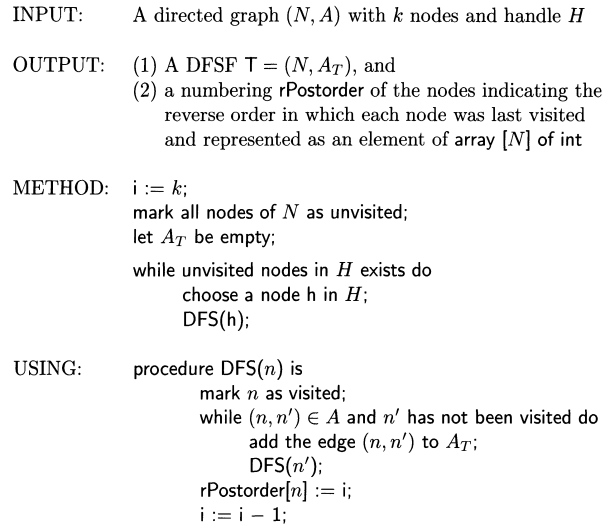
\includegraphics[scale=0.37]{dfsf.png}
\end{center}
\end{frame}
\begin{frame}{Example of DFSF Algorithm}
\begin{center}
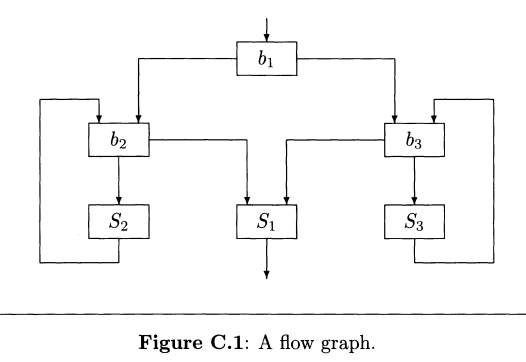
\includegraphics[scale=0.33]{dfsf1.png}

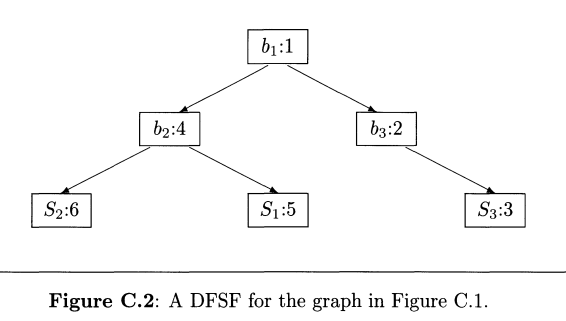
\includegraphics[scale=0.33]{dfsf2.png}
\end{center}
\end{frame}
\begin{frame}{Properties of Reverse Postorder}
\textbf{Categories of edges:}
\begin{itemize}
\item Tree edges: edges present in the spanning forest.
\item Forward edges: edges that are not tree edges and that go from a node to a proper descendant in the tree.
\item Back edges: edges that go from descendants to ancestors, incluing self-loops.
\item Cross edges: edges that go between nodes that are unrelated by the ancestor and descendant relations.
\end{itemize}
\end{frame}
\begin{frame}{Properties of Reverse Postorder}
\begin{center}
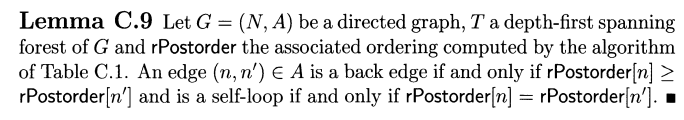
\includegraphics[scale=0.45]{lemmac9.png}

\end{center}
\textbf{Proof idea:} 
\begin{itemize}
\item Result of self loop is trivial.
\item 

``Only if'' direction can be obtained through the algorithm.

``If'' direction relys on a fact that there is no crossedge of the type.
\end{itemize}
\begin{center}
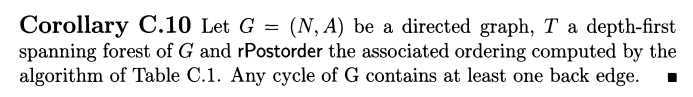
\includegraphics[scale=0.4]{co1.png}

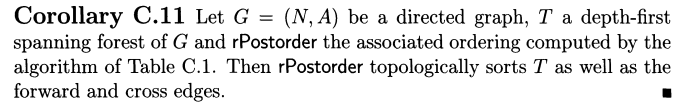
\includegraphics[scale=0.4]{co2.png}
\end{center}
\end{frame}

\begin{frame}{Loop Connectedness}
\begin{itemize}
\item The loop connectedness of $G$ with respect to a DFSF $T$ is the largest number of back edges found in any cycle-free path of $G$. Write as $d(G)$.
\item 

Dominator-back edge $(n_1, n_2)$.

\item 
Reducible graph: A directed graph with handle $H$ is reducible iff $(N, A\backslash A_{db})$ is acyclic and $H$ is still a handle.
\end{itemize}

\begin{center}
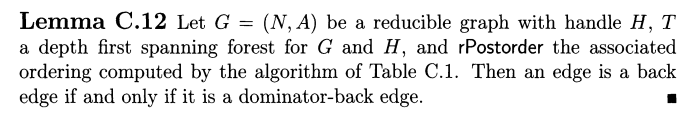
\includegraphics[scale=0.4]{lemmac12.png}

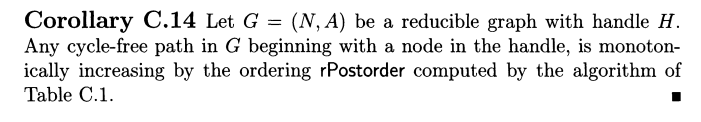
\includegraphics[scale=0.4]{lemmac14.png}
\end{center}
\end{frame}

\begin{frame}
\begin{center}
\Large
\textbf{Part III: Different Iterating Methods}
\end{center}

\end{frame}

\begin{frame}{Iterating in Reverse Postorder}
To concretize the algorithm, we can use FIFO or LIFO to instantiate the worklist.

\begin{center}
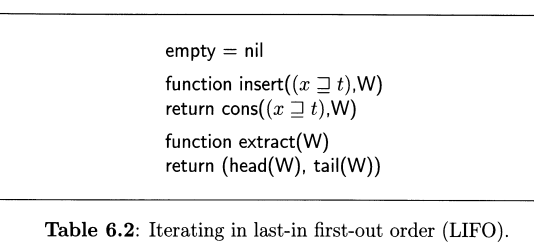
\includegraphics[scale=0.45]{fifo.png}
\end{center}
\end{frame}
\begin{frame}{Iterating in Reverse Postorder}
\begin{center}
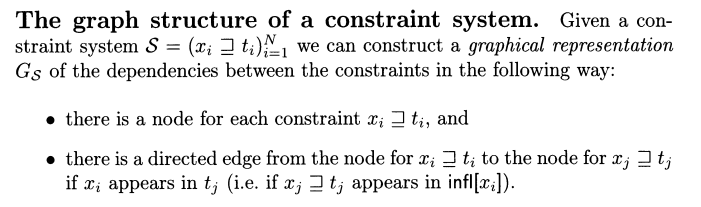
\includegraphics[scale=0.45]{graphderf.png}


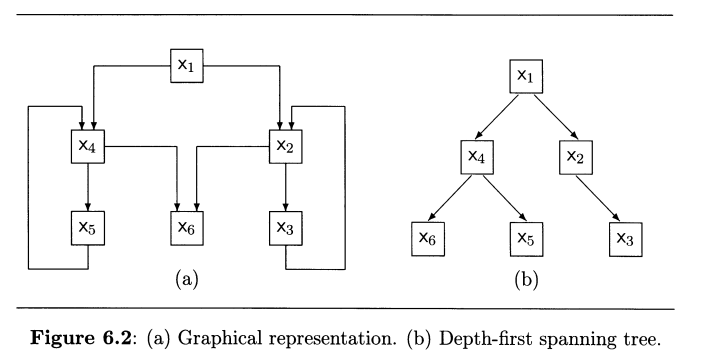
\includegraphics[scale=0.33]{gexp.png}
\end{center}
\end{frame}

\begin{frame}{Modify the Algorithm}
The working list will be splitted into two list: current list $\texttt{W.c}$ and pending list $\texttt{W.p}$.

\begin{center}
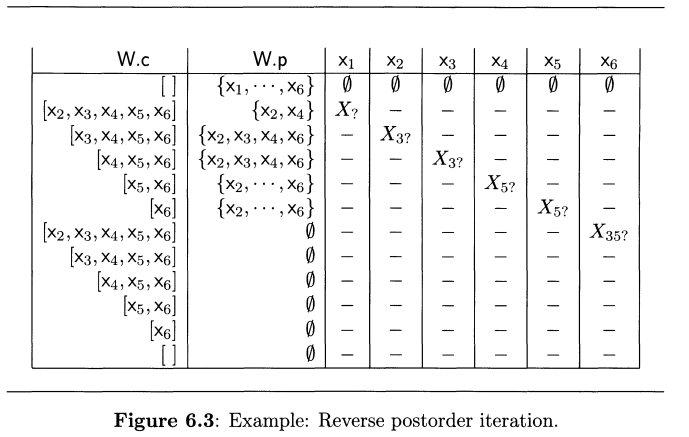
\includegraphics[scale=0.45]{rpe.png}
\end{center}
\end{frame}

\begin{frame}{Comparison with LIFO}
\begin{center}
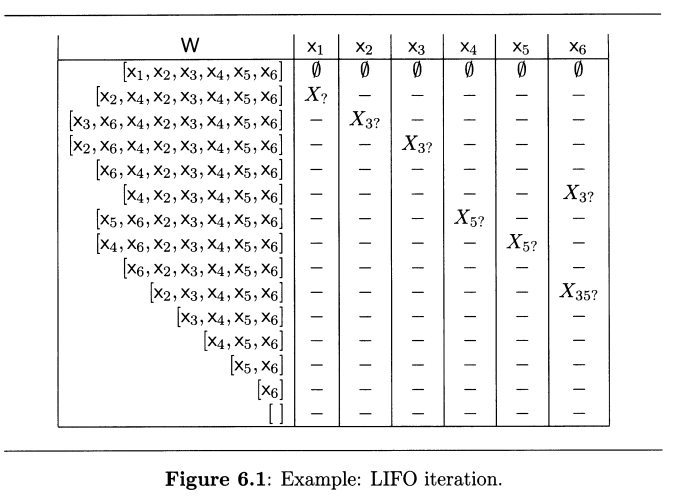
\includegraphics[scale=0.45]{lifotable.png}
\end{center}
\end{frame}

\begin{frame}{Round Robin Algorithm}
\begin{center}
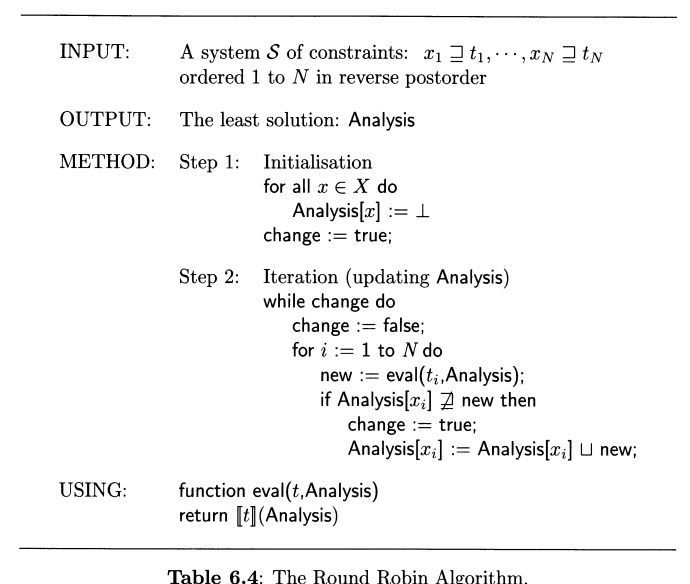
\includegraphics[scale=0.35]{robin.png}
\end{center}
\end{frame}

\begin{frame}{Theoretical Properties}
\begin{center}
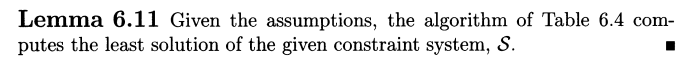
\includegraphics[scale=0.45]{lemma611.png}


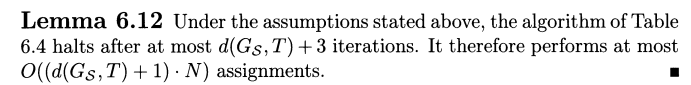
\includegraphics[scale=0.45]{lemma612.png}
\end{center}

Proof idea of Lemma 6.12:

A path contain $d$ back edges will cause the while loop in step 2 to iterate at most $d + 1$ times.

Overall bound: $O((d + 1)\cdot b)$, where $b$ is the number of the basic blocks.


\end{frame}

\begin{frame}{Iterating through Strong Components}
\begin{itemize}
\item 
\textbf{The algorithm:} SCCs are visited in topological order and within each SCC the nodes will be visited in reverse postorder.
\item 
Outer loop, intermediate loop and inner loop.
\item 
Priority of the constraint is obtained by pairs like $(scc, rp)$.
\end{itemize}
\end{frame}
\end{document}